	\begin{apendicesenv}
	
	% Imprime uma página indicando o início dos apêndices
	\partapendices
	\chapter{Mais detalhes sobre os experimentos}
			\begin{center}
	\newcommand{\mc}[3]{\multicolumn{#1}{#2}{#3}}
	\definecolor{tcB}{rgb}{0.447059,0.74902,0.266667}
	\definecolor{tcA}{rgb}{0.65098,0.65098,0.65098}
	\definecolor{tcC}{rgb}{1,0.94902,0}
	
	\begin{longtable}{|p{0.25\linewidth}|p{0.25\linewidth}|p{0.25\linewidth}|p{0.25\linewidth}|p{0.25\linewidth}|}

		% Columns headers
		\hline
		\mc{1}{|>{\columncolor{tcA}}c|}{Mel/Bark}&\mc{1}{|>{\columncolor{tcA}}c|}{Wavelet}&\mc{1}{|>{\columncolor{tcA}}c|}{G1}&\mc{1}{|>{\columncolor{tcA}}c|}{G2}&\mc{1}{|>{\columncolor{tcA}}c|}{Distance to (1,0)}\\\hline
		\endfirsthead
		
		\mc{2}{c}{{\tablename\ \thetable -- continued from previous page}} \\\hline
		% Columns headers
		\mc{1}{|>{\columncolor{tcA}}c|}{Mel/Bark}&\mc{1}{|>{\columncolor{tcA}}c|}{Wavelet}&\mc{1}{|>{\columncolor{tcA}}c|}{G1}&\mc{1}{|>{\columncolor{tcA}}c|}{G2}&\mc{1}{|>{\columncolor{tcA}}c|}{Distance to (1,0)}\\\hline
		\endhead
		
		\hline \mc{2}{c}{{Continues on next page}} \\
		\endfoot
		\endlastfoot

		\mc{1}{|>{\columncolor{tcB}}c|}{MEL}&\mc{1}{|>{\columncolor{tcB}}c|}{daub68}&\mc{1}{|>{\columncolor{tcB}}c|}{-0.81987033518}&\mc{1}{|>{\columncolor{tcB}}c|}{0.16859973133}&\mc{1}{|>{\columncolor{tcB}}c|}{1.8276635101}\\\hline
		\mc{1}{|>{\columncolor{tcC}}c|}{MEL}&\mc{1}{|>{\columncolor{tcC}}c|}{daub66}&\mc{1}{|>{\columncolor{tcC}}c|}{-0.82275683686}&\mc{1}{|>{\columncolor{tcC}}c|}{0.17347376181}&\mc{1}{|>{\columncolor{tcC}}c|}{1.8309930727}\\\hline
		\mc{1}{|>{\columncolor{tcC}}c|}{MEL}&\mc{1}{|>{\columncolor{tcC}}c|}{daub46}&\mc{1}{|>{\columncolor{tcC}}c|}{-0.82442762582}&\mc{1}{|>{\columncolor{tcC}}c|}{0.1684770305}&\mc{1}{|>{\columncolor{tcC}}c|}{1.8321901298}\\\hline
		\mc{1}{|>{\columncolor{tcC}}c|}{MEL}&\mc{1}{|>{\columncolor{tcC}}c|}{daub38}&\mc{1}{|>{\columncolor{tcC}}c|}{-0.82943741355}&\mc{1}{|>{\columncolor{tcC}}c|}{0.16191513634}&\mc{1}{|>{\columncolor{tcC}}c|}{1.8365886206}\\\hline
		\mc{1}{|>{\columncolor{tcC}}c|}{MEL}&\mc{1}{|>{\columncolor{tcC}}c|}{daub56}&\mc{1}{|>{\columncolor{tcC}}c|}{-0.82985884242}&\mc{1}{|>{\columncolor{tcC}}c|}{0.16282408441}&\mc{1}{|>{\columncolor{tcC}}c|}{1.8370887474}\\\hline
		\mc{1}{|>{\columncolor{tcC}}c|}{MEL}&\mc{1}{|>{\columncolor{tcC}}c|}{sym32}&\mc{1}{|>{\columncolor{tcC}}c|}{-0.83140702213}&\mc{1}{|>{\columncolor{tcC}}c|}{0.15928033929}&\mc{1}{|>{\columncolor{tcC}}c|}{1.8383204038}\\\hline
		\mc{1}{|>{\columncolor{tcC}}c|}{MEL}&\mc{1}{|>{\columncolor{tcC}}c|}{daub58}&\mc{1}{|>{\columncolor{tcC}}c|}{-0.83444401235}&\mc{1}{|>{\columncolor{tcC}}c|}{0.15579989008}&\mc{1}{|>{\columncolor{tcC}}c|}{1.8410481906}\\\hline
		\mc{1}{|>{\columncolor{tcC}}c|}{MEL}&\mc{1}{|>{\columncolor{tcC}}c|}{daub76}&\mc{1}{|>{\columncolor{tcC}}c|}{-0.83438273211}&\mc{1}{|>{\columncolor{tcC}}c|}{0.16029576013}&\mc{1}{|>{\columncolor{tcC}}c|}{1.841373058 }\\\hline
		\mc{1}{|>{\columncolor{tcC}}c|}{MEL}&\mc{1}{|>{\columncolor{tcC}}c|}{daub50}&\mc{1}{|>{\columncolor{tcC}}c|}{-0.8360988819}&\mc{1}{|>{\columncolor{tcC}}c|}{0.15569712697}&\mc{1}{|>{\columncolor{tcC}}c|}{1.8426884434}\\\hline
		\mc{1}{|>{\columncolor{tcC}}c|}{MEL}&\mc{1}{|>{\columncolor{tcC}}c|}{daub44}&\mc{1}{|>{\columncolor{tcC}}c|}{-0.83876290061}&\mc{1}{|>{\columncolor{tcC}}c|}{0.15635905061}&\mc{1}{|>{\columncolor{tcC}}c|}{1.8453989155}\\\hline
		\mc{1}{|>{\columncolor{tcC}}c|}{MEL}&\mc{1}{|>{\columncolor{tcC}}c|}{daub54}&\mc{1}{|>{\columncolor{tcC}}c|}{-0.83969908442}&\mc{1}{|>{\columncolor{tcC}}c|}{0.14943617057}&\mc{1}{|>{\columncolor{tcC}}c|}{1.845758351 }\\\hline
		\mc{1}{|>{\columncolor{tcC}}c|}{MEL}&\mc{1}{|>{\columncolor{tcC}}c|}{daub72}&\mc{1}{|>{\columncolor{tcC}}c|}{-0.84216780026}&\mc{1}{|>{\columncolor{tcC}}c|}{0.15361933943}&\mc{1}{|>{\columncolor{tcC}}c|}{1.8485619021}\\\hline
		\mc{1}{|>{\columncolor{tcC}}c|}{MEL}&\mc{1}{|>{\columncolor{tcC}}c|}{daub74}&\mc{1}{|>{\columncolor{tcC}}c|}{-0.84217451345}&\mc{1}{|>{\columncolor{tcC}}c|}{0.15405608522}&\mc{1}{|>{\columncolor{tcC}}c|}{1.8486049376}\\\hline
		\mc{1}{|>{\columncolor{tcC}}c|}{MEL}&\mc{1}{|>{\columncolor{tcC}}c|}{daub40}&\mc{1}{|>{\columncolor{tcC}}c|}{-0.8441972741}&\mc{1}{|>{\columncolor{tcC}}c|}{0.14626835783}&\mc{1}{|>{\columncolor{tcC}}c|}{1.8499886536}\\\hline
		\mc{1}{|>{\columncolor{tcC}}c|}{MEL}&\mc{1}{|>{\columncolor{tcC}}c|}{daub30}&\mc{1}{|>{\columncolor{tcC}}c|}{-0.84659101438}&\mc{1}{|>{\columncolor{tcC}}c|}{0.14697883041}&\mc{1}{|>{\columncolor{tcC}}c|}{1.8524311461}\\\hline
		\mc{1}{|>{\columncolor{tcC}}c|}{MEL}&\mc{1}{|>{\columncolor{tcC}}c|}{vaidyanathan24}&\mc{1}{|>{\columncolor{tcC}}c|}{-0.85025283499}&\mc{1}{|>{\columncolor{tcC}}c|}{0.14154317388}&\mc{1}{|>{\columncolor{tcC}}c|}{1.8556589189}\\\hline
		\mc{1}{|>{\columncolor{tcC}}c|}{MEL}&\mc{1}{|>{\columncolor{tcC}}c|}{daub22}&\mc{1}{|>{\columncolor{tcC}}c|}{-0.85347033723}&\mc{1}{|>{\columncolor{tcC}}c|}{0.13389108184}&\mc{1}{|>{\columncolor{tcC}}c|}{1.8583000599}\\\hline
		\mc{1}{|>{\columncolor{tcC}}c|}{MEL}&\mc{1}{|>{\columncolor{tcC}}c|}{daub64}&\mc{1}{|>{\columncolor{tcC}}c|}{-0.85506691345}&\mc{1}{|>{\columncolor{tcC}}c|}{0.13916811981}&\mc{1}{|>{\columncolor{tcC}}c|}{1.8602798228}\\\hline
		\mc{1}{|>{\columncolor{tcC}}c|}{MEL}&\mc{1}{|>{\columncolor{tcC}}c|}{daub32}&\mc{1}{|>{\columncolor{tcC}}c|}{-0.85583705232}&\mc{1}{|>{\columncolor{tcC}}c|}{0.13795452196}&\mc{1}{|>{\columncolor{tcC}}c|}{1.8609574457}\\\hline
		\mc{1}{|>{\columncolor{tcC}}c|}{MEL}&\mc{1}{|>{\columncolor{tcC}}c|}{daub62}&\mc{1}{|>{\columncolor{tcC}}c|}{-0.85822199875}&\mc{1}{|>{\columncolor{tcC}}c|}{0.13313055114}&\mc{1}{|>{\columncolor{tcC}}c|}{1.8629849007}\\\hline
		\mc{1}{|>{\columncolor{tcC}}c|}{MEL}&\mc{1}{|>{\columncolor{tcC}}c|}{daub36}&\mc{1}{|>{\columncolor{tcC}}c|}{-0.85905493715}&\mc{1}{|>{\columncolor{tcC}}c|}{0.13074550631}&\mc{1}{|>{\columncolor{tcC}}c|}{1.8636468675}\\\hline
		\mc{1}{|>{\columncolor{tcC}}c|}{MEL}&\mc{1}{|>{\columncolor{tcC}}c|}{daub60}&\mc{1}{|>{\columncolor{tcC}}c|}{-0.85902689237}&\mc{1}{|>{\columncolor{tcC}}c|}{0.13321257548}&\mc{1}{|>{\columncolor{tcC}}c|}{1.8637935982}\\\hline
		\mc{1}{|>{\columncolor{tcC}}c|}{MEL}&\mc{1}{|>{\columncolor{tcC}}c|}{daub70}&\mc{1}{|>{\columncolor{tcC}}c|}{-0.85961195775}&\mc{1}{|>{\columncolor{tcC}}c|}{0.13351442806}&\mc{1}{|>{\columncolor{tcC}}c|}{1.8643987599}\\\hline
		\mc{1}{|>{\columncolor{tcC}}c|}{BARK}&\mc{1}{|>{\columncolor{tcC}}c|}{daub72}&\mc{1}{|>{\columncolor{tcC}}c|}{-0.86227613205}&\mc{1}{|>{\columncolor{tcC}}c|}{0.10510191673}&\mc{1}{|>{\columncolor{tcC}}c|}{1.8652396106}\\\hline
		\mc{1}{|>{\columncolor{tcC}}c|}{MEL}&\mc{1}{|>{\columncolor{tcC}}c|}{daub24}&\mc{1}{|>{\columncolor{tcC}}c|}{-0.86425347657}&\mc{1}{|>{\columncolor{tcC}}c|}{0.12621215536}&\mc{1}{|>{\columncolor{tcC}}c|}{1.868520948 }\\\hline
		\mc{1}{|>{\columncolor{tcC}}c|}{MEL}&\mc{1}{|>{\columncolor{tcC}}c|}{beylkin18}&\mc{1}{|>{\columncolor{tcC}}c|}{-0.86663968015}&\mc{1}{|>{\columncolor{tcC}}c|}{0.12227384535}&\mc{1}{|>{\columncolor{tcC}}c|}{1.8706401548}\\\hline
		\mc{1}{|>{\columncolor{tcC}}c|}{MEL}&\mc{1}{|>{\columncolor{tcC}}c|}{haar}&\mc{1}{|>{\columncolor{tcC}}c|}{-0.8751287703}&\mc{1}{|>{\columncolor{tcC}}c|}{0.10425038712}&\mc{1}{|>{\columncolor{tcC}}c|}{1.8780245069}\\\hline
		\mc{1}{|>{\columncolor{tcC}}c|}{MEL}&\mc{1}{|>{\columncolor{tcC}}c|}{daub42}&\mc{1}{|>{\columncolor{tcC}}c|}{-0.87549124907}&\mc{1}{|>{\columncolor{tcC}}c|}{0.11364400592}&\mc{1}{|>{\columncolor{tcC}}c|}{1.8789311817}\\\hline
		\mc{1}{|>{\columncolor{tcC}}c|}{MEL}&\mc{1}{|>{\columncolor{tcC}}c|}{daub52}&\mc{1}{|>{\columncolor{tcC}}c|}{-0.87964315202}&\mc{1}{|>{\columncolor{tcC}}c|}{0.11481361073}&\mc{1}{|>{\columncolor{tcC}}c|}{1.8831464479}\\\hline
		\mc{1}{|>{\columncolor{tcC}}c|}{MEL}&\mc{1}{|>{\columncolor{tcC}}c|}{daub26}&\mc{1}{|>{\columncolor{tcC}}c|}{-0.88060441409}&\mc{1}{|>{\columncolor{tcC}}c|}{0.10742219345}&\mc{1}{|>{\columncolor{tcC}}c|}{1.8836699525}\\\hline
		\mc{1}{|>{\columncolor{tcC}}c|}{MEL}&\mc{1}{|>{\columncolor{tcC}}c|}{coif6}&\mc{1}{|>{\columncolor{tcC}}c|}{-0.88139412664}&\mc{1}{|>{\columncolor{tcC}}c|}{0.096654653849}&\mc{1}{|>{\columncolor{tcC}}c|}{1.8838752564}\\\hline
		\mc{1}{|>{\columncolor{tcC}}c|}{MEL}&\mc{1}{|>{\columncolor{tcC}}c|}{daub48}&\mc{1}{|>{\columncolor{tcC}}c|}{-0.884494971}&\mc{1}{|>{\columncolor{tcC}}c|}{0.10464028399}&\mc{1}{|>{\columncolor{tcC}}c|}{1.8873979137}\\\hline
		\mc{1}{|>{\columncolor{tcC}}c|}{MEL}&\mc{1}{|>{\columncolor{tcC}}c|}{coif12}&\mc{1}{|>{\columncolor{tcC}}c|}{-0.88621810741}&\mc{1}{|>{\columncolor{tcC}}c|}{0.10713000789}&\mc{1}{|>{\columncolor{tcC}}c|}{1.8892579462}\\\hline
		\mc{1}{|>{\columncolor{tcC}}c|}{BARK}&\mc{1}{|>{\columncolor{tcC}}c|}{daub38}&\mc{1}{|>{\columncolor{tcC}}c|}{-0.88799800935}&\mc{1}{|>{\columncolor{tcC}}c|}{0.083648332109}&\mc{1}{|>{\columncolor{tcC}}c|}{1.8898501334}\\\hline
		\mc{1}{|>{\columncolor{tcC}}c|}{BARK}&\mc{1}{|>{\columncolor{tcC}}c|}{daub30}&\mc{1}{|>{\columncolor{tcC}}c|}{-0.88972476619}&\mc{1}{|>{\columncolor{tcC}}c|}{0.085376859831}&\mc{1}{|>{\columncolor{tcC}}c|}{1.8916524258}\\\hline
		\mc{1}{|>{\columncolor{tcC}}c|}{MEL}&\mc{1}{|>{\columncolor{tcC}}c|}{daub18}&\mc{1}{|>{\columncolor{tcC}}c|}{-0.89097834069}&\mc{1}{|>{\columncolor{tcC}}c|}{0.095274430933}&\mc{1}{|>{\columncolor{tcC}}c|}{1.8933769572}\\\hline
		\mc{1}{|>{\columncolor{tcC}}c|}{BARK}&\mc{1}{|>{\columncolor{tcC}}c|}{sym16}&\mc{1}{|>{\columncolor{tcC}}c|}{-0.89411001896}&\mc{1}{|>{\columncolor{tcC}}c|}{0.074284289987}&\mc{1}{|>{\columncolor{tcC}}c|}{1.8955661211}\\\hline
		\mc{1}{|>{\columncolor{tcC}}c|}{MEL}&\mc{1}{|>{\columncolor{tcC}}c|}{daub14}&\mc{1}{|>{\columncolor{tcC}}c|}{-0.89577746381}&\mc{1}{|>{\columncolor{tcC}}c|}{0.093136061688}&\mc{1}{|>{\columncolor{tcC}}c|}{1.8980638868}\\\hline
		\mc{1}{|>{\columncolor{tcC}}c|}{MEL}&\mc{1}{|>{\columncolor{tcC}}c|}{daub28}&\mc{1}{|>{\columncolor{tcC}}c|}{-0.89569679017}&\mc{1}{|>{\columncolor{tcC}}c|}{0.098981702073}&\mc{1}{|>{\columncolor{tcC}}c|}{1.8982791411}\\\hline
		\mc{1}{|>{\columncolor{tcC}}c|}{MEL}&\mc{1}{|>{\columncolor{tcC}}c|}{coif30}&\mc{1}{|>{\columncolor{tcC}}c|}{-0.89832116907}&\mc{1}{|>{\columncolor{tcC}}c|}{0.093031380818}&\mc{1}{|>{\columncolor{tcC}}c|}{1.9005994051}\\\hline
		\mc{1}{|>{\columncolor{tcC}}c|}{MEL}&\mc{1}{|>{\columncolor{tcC}}c|}{sym16}&\mc{1}{|>{\columncolor{tcC}}c|}{-0.90015330494}&\mc{1}{|>{\columncolor{tcC}}c|}{0.083660442286}&\mc{1}{|>{\columncolor{tcC}}c|}{1.9019941251}\\\hline
		\mc{1}{|>{\columncolor{tcC}}c|}{BARK}&\mc{1}{|>{\columncolor{tcC}}c|}{daub58}&\mc{1}{|>{\columncolor{tcC}}c|}{-0.90073238727}&\mc{1}{|>{\columncolor{tcC}}c|}{0.072743222484}&\mc{1}{|>{\columncolor{tcC}}c|}{1.9021238615}\\\hline
		\mc{1}{|>{\columncolor{tcC}}c|}{MEL}&\mc{1}{|>{\columncolor{tcC}}c|}{daub16}&\mc{1}{|>{\columncolor{tcC}}c|}{-0.90144036946}&\mc{1}{|>{\columncolor{tcC}}c|}{0.087694885531}&\mc{1}{|>{\columncolor{tcC}}c|}{1.9034615498}\\\hline
		\mc{1}{|>{\columncolor{tcC}}c|}{MEL}&\mc{1}{|>{\columncolor{tcC}}c|}{daub8}&\mc{1}{|>{\columncolor{tcC}}c|}{-0.90909811878}&\mc{1}{|>{\columncolor{tcC}}c|}{0.077819841306}&\mc{1}{|>{\columncolor{tcC}}c|}{1.9106835308}\\\hline
		\mc{1}{|>{\columncolor{tcC}}c|}{MEL}&\mc{1}{|>{\columncolor{tcC}}c|}{coif24}&\mc{1}{|>{\columncolor{tcC}}c|}{-0.91003378885}&\mc{1}{|>{\columncolor{tcC}}c|}{0.077549359705}&\mc{1}{|>{\columncolor{tcC}}c|}{1.911607433 }\\\hline
		\mc{1}{|>{\columncolor{tcC}}c|}{BARK}&\mc{1}{|>{\columncolor{tcC}}c|}{daub34}&\mc{1}{|>{\columncolor{tcC}}c|}{-0.91070674003}&\mc{1}{|>{\columncolor{tcC}}c|}{0.065512772167}&\mc{1}{|>{\columncolor{tcC}}c|}{1.9118295347}\\\hline
		\mc{1}{|>{\columncolor{tcC}}c|}{MEL}&\mc{1}{|>{\columncolor{tcC}}c|}{daub20}&\mc{1}{|>{\columncolor{tcC}}c|}{-0.90997470357}&\mc{1}{|>{\columncolor{tcC}}c|}{0.085812436124}&\mc{1}{|>{\columncolor{tcC}}c|}{1.9119014468}\\\hline
		\mc{1}{|>{\columncolor{tcC}}c|}{MEL}&\mc{1}{|>{\columncolor{tcC}}c|}{daub6}&\mc{1}{|>{\columncolor{tcC}}c|}{-0.91020526551}&\mc{1}{|>{\columncolor{tcC}}c|}{0.08136901387}&\mc{1}{|>{\columncolor{tcC}}c|}{1.911937518 }\\\hline
		\mc{1}{|>{\columncolor{tcC}}c|}{BARK}&\mc{1}{|>{\columncolor{tcC}}c|}{daub48}&\mc{1}{|>{\columncolor{tcC}}c|}{-0.91164281148}&\mc{1}{|>{\columncolor{tcC}}c|}{0.064170196652}&\mc{1}{|>{\columncolor{tcC}}c|}{1.9127195437}\\\hline
		\mc{1}{|>{\columncolor{tcC}}c|}{MEL}&\mc{1}{|>{\columncolor{tcC}}c|}{daub4}&\mc{1}{|>{\columncolor{tcC}}c|}{-0.91194809545}&\mc{1}{|>{\columncolor{tcC}}c|}{0.074748135147}&\mc{1}{|>{\columncolor{tcC}}c|}{1.913408687 }\\\hline
		\mc{1}{|>{\columncolor{tcC}}c|}{BARK}&\mc{1}{|>{\columncolor{tcC}}c|}{daub18}&\mc{1}{|>{\columncolor{tcC}}c|}{-0.91280395947}&\mc{1}{|>{\columncolor{tcC}}c|}{0.051525308818}&\mc{1}{|>{\columncolor{tcC}}c|}{1.9134978037}\\\hline
		\mc{1}{|>{\columncolor{tcC}}c|}{MEL}&\mc{1}{|>{\columncolor{tcC}}c|}{daub10}&\mc{1}{|>{\columncolor{tcC}}c|}{-0.91271891559}&\mc{1}{|>{\columncolor{tcC}}c|}{0.073312126539}&\mc{1}{|>{\columncolor{tcC}}c|}{1.9141233811}\\\hline
		\mc{1}{|>{\columncolor{tcC}}c|}{BARK}&\mc{1}{|>{\columncolor{tcC}}c|}{daub8}&\mc{1}{|>{\columncolor{tcC}}c|}{-0.91559722851}&\mc{1}{|>{\columncolor{tcC}}c|}{0.048528787755}&\mc{1}{|>{\columncolor{tcC}}c|}{1.916211832 }\\\hline
		\mc{1}{|>{\columncolor{tcC}}c|}{MEL}&\mc{1}{|>{\columncolor{tcC}}c|}{coif18}&\mc{1}{|>{\columncolor{tcC}}c|}{-0.91555531429}&\mc{1}{|>{\columncolor{tcC}}c|}{0.074023399675}&\mc{1}{|>{\columncolor{tcC}}c|}{1.9169850354}\\\hline
		\mc{1}{|>{\columncolor{tcC}}c|}{BARK}&\mc{1}{|>{\columncolor{tcC}}c|}{coif18}&\mc{1}{|>{\columncolor{tcC}}c|}{-0.91675224423}&\mc{1}{|>{\columncolor{tcC}}c|}{0.057231495604}&\mc{1}{|>{\columncolor{tcC}}c|}{1.9176064794}\\\hline
		\mc{1}{|>{\columncolor{tcC}}c|}{BARK}&\mc{1}{|>{\columncolor{tcC}}c|}{daub36}&\mc{1}{|>{\columncolor{tcC}}c|}{-0.92212838315}&\mc{1}{|>{\columncolor{tcC}}c|}{0.057444787581}&\mc{1}{|>{\columncolor{tcC}}c|}{1.9229865899}\\\hline
		\mc{1}{|>{\columncolor{tcC}}c|}{MEL}&\mc{1}{|>{\columncolor{tcC}}c|}{daub12}&\mc{1}{|>{\columncolor{tcC}}c|}{-0.92207646297}&\mc{1}{|>{\columncolor{tcC}}c|}{0.061072095791}&\mc{1}{|>{\columncolor{tcC}}c|}{1.9230464712}\\\hline
		\mc{1}{|>{\columncolor{tcC}}c|}{BARK}&\mc{1}{|>{\columncolor{tcC}}c|}{daub76}&\mc{1}{|>{\columncolor{tcC}}c|}{-0.92292899256}&\mc{1}{|>{\columncolor{tcC}}c|}{0.050140113129}&\mc{1}{|>{\columncolor{tcC}}c|}{1.9235825798}\\\hline
		\mc{1}{|>{\columncolor{tcC}}c|}{BARK}&\mc{1}{|>{\columncolor{tcC}}c|}{daub66}&\mc{1}{|>{\columncolor{tcC}}c|}{-0.92315084259}&\mc{1}{|>{\columncolor{tcC}}c|}{0.059572734647}&\mc{1}{|>{\columncolor{tcC}}c|}{1.9240733027}\\\hline
		\mc{1}{|>{\columncolor{tcC}}c|}{BARK}&\mc{1}{|>{\columncolor{tcC}}c|}{coif12}&\mc{1}{|>{\columncolor{tcC}}c|}{-0.92439876216}&\mc{1}{|>{\columncolor{tcC}}c|}{0.047958961415}&\mc{1}{|>{\columncolor{tcC}}c|}{1.9249962747}\\\hline
		\mc{1}{|>{\columncolor{tcC}}c|}{BARK}&\mc{1}{|>{\columncolor{tcC}}c|}{sym32}&\mc{1}{|>{\columncolor{tcC}}c|}{-0.92475467742}&\mc{1}{|>{\columncolor{tcC}}c|}{0.043131501444}&\mc{1}{|>{\columncolor{tcC}}c|}{1.92523788  }\\\hline
		\mc{1}{|>{\columncolor{tcC}}c|}{MEL}&\mc{1}{|>{\columncolor{tcC}}c|}{sym8}&\mc{1}{|>{\columncolor{tcC}}c|}{-0.92508512068}&\mc{1}{|>{\columncolor{tcC}}c|}{0.061611109917}&\mc{1}{|>{\columncolor{tcC}}c|}{1.9260707803}\\\hline
		\mc{1}{|>{\columncolor{tcC}}c|}{BARK}&\mc{1}{|>{\columncolor{tcC}}c|}{daub44}&\mc{1}{|>{\columncolor{tcC}}c|}{-0.92554648241}&\mc{1}{|>{\columncolor{tcC}}c|}{0.049860021654}&\mc{1}{|>{\columncolor{tcC}}c|}{1.9261919109}\\\hline
		\mc{1}{|>{\columncolor{tcC}}c|}{BARK}&\mc{1}{|>{\columncolor{tcC}}c|}{daub50}&\mc{1}{|>{\columncolor{tcC}}c|}{-0.92538783066}&\mc{1}{|>{\columncolor{tcC}}c|}{0.061400787223}&\mc{1}{|>{\columncolor{tcC}}c|}{1.9263666201}\\\hline
		\mc{1}{|>{\columncolor{tcC}}c|}{MEL}&\mc{1}{|>{\columncolor{tcC}}c|}{daub34}&\mc{1}{|>{\columncolor{tcC}}c|}{-0.92532666722}&\mc{1}{|>{\columncolor{tcC}}c|}{0.065582423691}&\mc{1}{|>{\columncolor{tcC}}c|}{1.9264433108}\\\hline
		\mc{1}{|>{\columncolor{tcC}}c|}{BARK}&\mc{1}{|>{\columncolor{tcC}}c|}{daub70}&\mc{1}{|>{\columncolor{tcC}}c|}{-0.92672937192}&\mc{1}{|>{\columncolor{tcC}}c|}{0.055892579296}&\mc{1}{|>{\columncolor{tcC}}c|}{1.9275398966}\\\hline
		\mc{1}{|>{\columncolor{tcC}}c|}{BARK}&\mc{1}{|>{\columncolor{tcC}}c|}{daub74}&\mc{1}{|>{\columncolor{tcC}}c|}{-0.9281501735}&\mc{1}{|>{\columncolor{tcC}}c|}{0.041057143576}&\mc{1}{|>{\columncolor{tcC}}c|}{1.9285872499}\\\hline
		\mc{1}{|>{\columncolor{tcC}}c|}{BARK}&\mc{1}{|>{\columncolor{tcC}}c|}{daub42}&\mc{1}{|>{\columncolor{tcC}}c|}{-0.92811582564}&\mc{1}{|>{\columncolor{tcC}}c|}{0.062026450784}&\mc{1}{|>{\columncolor{tcC}}c|}{1.9291132465}\\\hline
		\mc{1}{|>{\columncolor{tcC}}c|}{BARK}&\mc{1}{|>{\columncolor{tcC}}c|}{daub24}&\mc{1}{|>{\columncolor{tcC}}c|}{-0.93435581993}&\mc{1}{|>{\columncolor{tcC}}c|}{0.043083204464}&\mc{1}{|>{\columncolor{tcC}}c|}{1.9348355487}\\\hline
		\mc{1}{|>{\columncolor{tcC}}c|}{BARK}&\mc{1}{|>{\columncolor{tcC}}c|}{daub46}&\mc{1}{|>{\columncolor{tcC}}c|}{-0.93676709759}&\mc{1}{|>{\columncolor{tcC}}c|}{0.048802008105}&\mc{1}{|>{\columncolor{tcC}}c|}{1.9373818483}\\\hline
		\mc{1}{|>{\columncolor{tcC}}c|}{BARK}&\mc{1}{|>{\columncolor{tcC}}c|}{daub68}&\mc{1}{|>{\columncolor{tcC}}c|}{-0.93741887176}&\mc{1}{|>{\columncolor{tcC}}c|}{0.043170559136}&\mc{1}{|>{\columncolor{tcC}}c|}{1.9378997863}\\\hline
		\mc{1}{|>{\columncolor{tcC}}c|}{BARK}&\mc{1}{|>{\columncolor{tcC}}c|}{daub28}&\mc{1}{|>{\columncolor{tcC}}c|}{-0.93908048105}&\mc{1}{|>{\columncolor{tcC}}c|}{0.040187811629}&\mc{1}{|>{\columncolor{tcC}}c|}{1.9394968864}\\\hline
		\mc{1}{|>{\columncolor{tcC}}c|}{BARK}&\mc{1}{|>{\columncolor{tcC}}c|}{daub22}&\mc{1}{|>{\columncolor{tcC}}c|}{-0.94434920743}&\mc{1}{|>{\columncolor{tcC}}c|}{0.035427215334}&\mc{1}{|>{\columncolor{tcC}}c|}{1.9446719333}\\\hline
		\mc{1}{|>{\columncolor{tcC}}c|}{BARK}&\mc{1}{|>{\columncolor{tcC}}c|}{daub12}&\mc{1}{|>{\columncolor{tcC}}c|}{-0.9463192249}&\mc{1}{|>{\columncolor{tcC}}c|}{0.026648254777}&\mc{1}{|>{\columncolor{tcC}}c|}{1.9465016452}\\\hline
		\mc{1}{|>{\columncolor{tcC}}c|}{BARK}&\mc{1}{|>{\columncolor{tcC}}c|}{daub52}&\mc{1}{|>{\columncolor{tcC}}c|}{-0.94723724495}&\mc{1}{|>{\columncolor{tcC}}c|}{0.034266820094}&\mc{1}{|>{\columncolor{tcC}}c|}{1.9475387295}\\\hline
		\mc{1}{|>{\columncolor{tcC}}c|}{BARK}&\mc{1}{|>{\columncolor{tcC}}c|}{daub16}&\mc{1}{|>{\columncolor{tcC}}c|}{-0.9472394768}&\mc{1}{|>{\columncolor{tcC}}c|}{0.035687352473}&\mc{1}{|>{\columncolor{tcC}}c|}{1.9475664731}\\\hline
		\mc{1}{|>{\columncolor{tcC}}c|}{BARK}&\mc{1}{|>{\columncolor{tcC}}c|}{daub54}&\mc{1}{|>{\columncolor{tcC}}c|}{-0.94856125453}&\mc{1}{|>{\columncolor{tcC}}c|}{0.035381834898}&\mc{1}{|>{\columncolor{tcC}}c|}{1.9488824585}\\\hline
		\mc{1}{|>{\columncolor{tcC}}c|}{BARK}&\mc{1}{|>{\columncolor{tcC}}c|}{daub10}&\mc{1}{|>{\columncolor{tcC}}c|}{-0.94866926208}&\mc{1}{|>{\columncolor{tcC}}c|}{0.029684396452}&\mc{1}{|>{\columncolor{tcC}}c|}{1.9488953426}\\\hline
		\mc{1}{|>{\columncolor{tcC}}c|}{BARK}&\mc{1}{|>{\columncolor{tcC}}c|}{daub64}&\mc{1}{|>{\columncolor{tcC}}c|}{-0.95062037297}&\mc{1}{|>{\columncolor{tcC}}c|}{0.040436537596}&\mc{1}{|>{\columncolor{tcC}}c|}{1.9510394545}\\\hline
		\mc{1}{|>{\columncolor{tcC}}c|}{BARK}&\mc{1}{|>{\columncolor{tcC}}c|}{coif24}&\mc{1}{|>{\columncolor{tcC}}c|}{-0.95422620541}&\mc{1}{|>{\columncolor{tcC}}c|}{0.034391680766}&\mc{1}{|>{\columncolor{tcC}}c|}{1.954528805 }\\\hline
		\mc{1}{|>{\columncolor{tcC}}c|}{BARK}&\mc{1}{|>{\columncolor{tcC}}c|}{daub60}&\mc{1}{|>{\columncolor{tcC}}c|}{-0.9543100896}&\mc{1}{|>{\columncolor{tcC}}c|}{0.029328121787}&\mc{1}{|>{\columncolor{tcC}}c|}{1.9545301392}\\\hline
		\mc{1}{|>{\columncolor{tcC}}c|}{BARK}&\mc{1}{|>{\columncolor{tcC}}c|}{daub6}&\mc{1}{|>{\columncolor{tcC}}c|}{-0.95610516142}&\mc{1}{|>{\columncolor{tcC}}c|}{0.02682166785}&\mc{1}{|>{\columncolor{tcC}}c|}{1.9562890391}\\\hline
		\mc{1}{|>{\columncolor{tcC}}c|}{BARK}&\mc{1}{|>{\columncolor{tcC}}c|}{daub40}&\mc{1}{|>{\columncolor{tcC}}c|}{-0.95707346752}&\mc{1}{|>{\columncolor{tcC}}c|}{0.028800516221}&\mc{1}{|>{\columncolor{tcC}}c|}{1.9572853719}\\\hline
		\mc{1}{|>{\columncolor{tcC}}c|}{BARK}&\mc{1}{|>{\columncolor{tcC}}c|}{daub56}&\mc{1}{|>{\columncolor{tcC}}c|}{-0.95747044532}&\mc{1}{|>{\columncolor{tcC}}c|}{0.032875083138}&\mc{1}{|>{\columncolor{tcC}}c|}{1.957746489 }\\\hline
		\mc{1}{|>{\columncolor{tcC}}c|}{BARK}&\mc{1}{|>{\columncolor{tcC}}c|}{daub20}&\mc{1}{|>{\columncolor{tcC}}c|}{-0.95794273071}&\mc{1}{|>{\columncolor{tcC}}c|}{0.017260521321}&\mc{1}{|>{\columncolor{tcC}}c|}{1.9580188105}\\\hline
		\mc{1}{|>{\columncolor{tcC}}c|}{BARK}&\mc{1}{|>{\columncolor{tcC}}c|}{daub4}&\mc{1}{|>{\columncolor{tcC}}c|}{-0.9601254027}&\mc{1}{|>{\columncolor{tcC}}c|}{0.0070493940482}&\mc{1}{|>{\columncolor{tcC}}c|}{1.9601380789}\\\hline
		\mc{1}{|>{\columncolor{tcC}}c|}{BARK}&\mc{1}{|>{\columncolor{tcC}}c|}{daub32}&\mc{1}{|>{\columncolor{tcC}}c|}{-0.96138618849}&\mc{1}{|>{\columncolor{tcC}}c|}{0.021947144843}&\mc{1}{|>{\columncolor{tcC}}c|}{1.9615089746}\\\hline
		\mc{1}{|>{\columncolor{tcC}}c|}{BARK}&\mc{1}{|>{\columncolor{tcC}}c|}{daub26}&\mc{1}{|>{\columncolor{tcC}}c|}{-0.96187673556}&\mc{1}{|>{\columncolor{tcC}}c|}{0.019424077449}&\mc{1}{|>{\columncolor{tcC}}c|}{1.9619728898}\\\hline
		\mc{1}{|>{\columncolor{tcC}}c|}{BARK}&\mc{1}{|>{\columncolor{tcC}}c|}{daub14}&\mc{1}{|>{\columncolor{tcC}}c|}{-0.96226158205}&\mc{1}{|>{\columncolor{tcC}}c|}{0.012636791936}&\mc{1}{|>{\columncolor{tcC}}c|}{1.9623022715}\\\hline
		\mc{1}{|>{\columncolor{tcC}}c|}{BARK}&\mc{1}{|>{\columncolor{tcC}}c|}{daub62}&\mc{1}{|>{\columncolor{tcC}}c|}{-0.96306376236}&\mc{1}{|>{\columncolor{tcC}}c|}{0.026062253896}&\mc{1}{|>{\columncolor{tcC}}c|}{1.9632367601}\\\hline
		\mc{1}{|>{\columncolor{tcC}}c|}{BARK}&\mc{1}{|>{\columncolor{tcC}}c|}{coif30}&\mc{1}{|>{\columncolor{tcC}}c|}{-0.9638082517}&\mc{1}{|>{\columncolor{tcC}}c|}{0.023081992204}&\mc{1}{|>{\columncolor{tcC}}c|}{1.9639438963}\\\hline
		\mc{1}{|>{\columncolor{tcC}}c|}{BARK}&\mc{1}{|>{\columncolor{tcC}}c|}{beylkin18}&\mc{1}{|>{\columncolor{tcC}}c|}{-0.96477497961}&\mc{1}{|>{\columncolor{tcC}}c|}{0.032481117949}&\mc{1}{|>{\columncolor{tcC}}c|}{1.9650434457}\\\hline
		\mc{1}{|>{\columncolor{tcC}}c|}{BARK}&\mc{1}{|>{\columncolor{tcC}}c|}{coif6}&\mc{1}{|>{\columncolor{tcC}}c|}{-0.97404005705}&\mc{1}{|>{\columncolor{tcC}}c|}{0.0069558779098}&\mc{1}{|>{\columncolor{tcC}}c|}{1.9740523121}\\\hline
		\mc{1}{|>{\columncolor{tcC}}c|}{BARK}&\mc{1}{|>{\columncolor{tcC}}c|}{vaidyanathan24}&\mc{1}{|>{\columncolor{tcC}}c|}{-0.9748210631}&\mc{1}{|>{\columncolor{tcC}}c|}{0.02304479056}&\mc{1}{|>{\columncolor{tcC}}c|}{1.9749555169}\\\hline
		\mc{1}{|>{\columncolor{tcC}}c|}{BARK}&\mc{1}{|>{\columncolor{tcC}}c|}{haar}&\mc{1}{|>{\columncolor{tcC}}c|}{-0.98344077802}&\mc{1}{|>{\columncolor{tcC}}c|}{-0.0029529731372}&\mc{1}{|>{\columncolor{tcC}}c|}{1.9834429762}\\\hline
		\mc{1}{|>{\columncolor{tcC}}c|}{BARK}&\mc{1}{|>{\columncolor{tcC}}c|}{sym8}&\mc{1}{|>{\columncolor{tcC}}c|}{-0.99142639503}&\mc{1}{|>{\columncolor{tcC}}c|}{-0.0042312730775}&\mc{1}{|>{\columncolor{tcC}}c|}{1.9914308902}\\\hline

		\caption{Wavelet \textit{x} Mel/Bark combination in the paraconsistent plane ordered by the distance from the paraconsistent (1,0) vertice.}
		\label{tab:distParacomFrom10BarkAndMel}
	\end{longtable}
\end{center}
			\begin{landscape}
					\begin{figure}[h]
						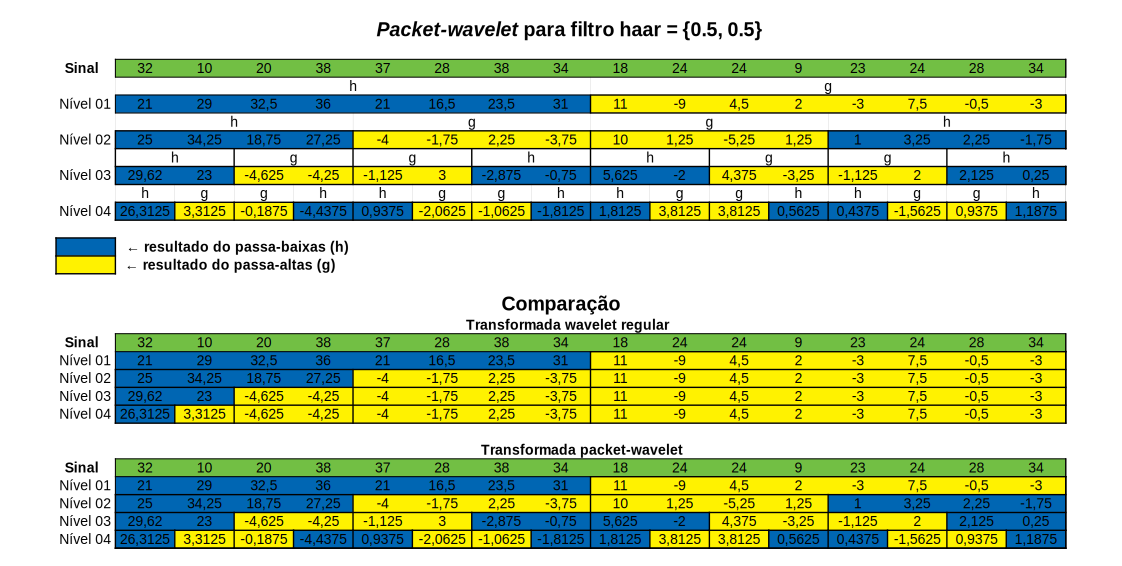
\includegraphics[width=1\linewidth]{images/haarWaveletExamples.pdf}
						\caption{Demostração numérica das transformadas Wavelet e Wavelet packet}
						\label{fig:haarWaveletExamples}
					\end{figure}
			\end{landscape}
			\begin{figure}[h]
				\centering
				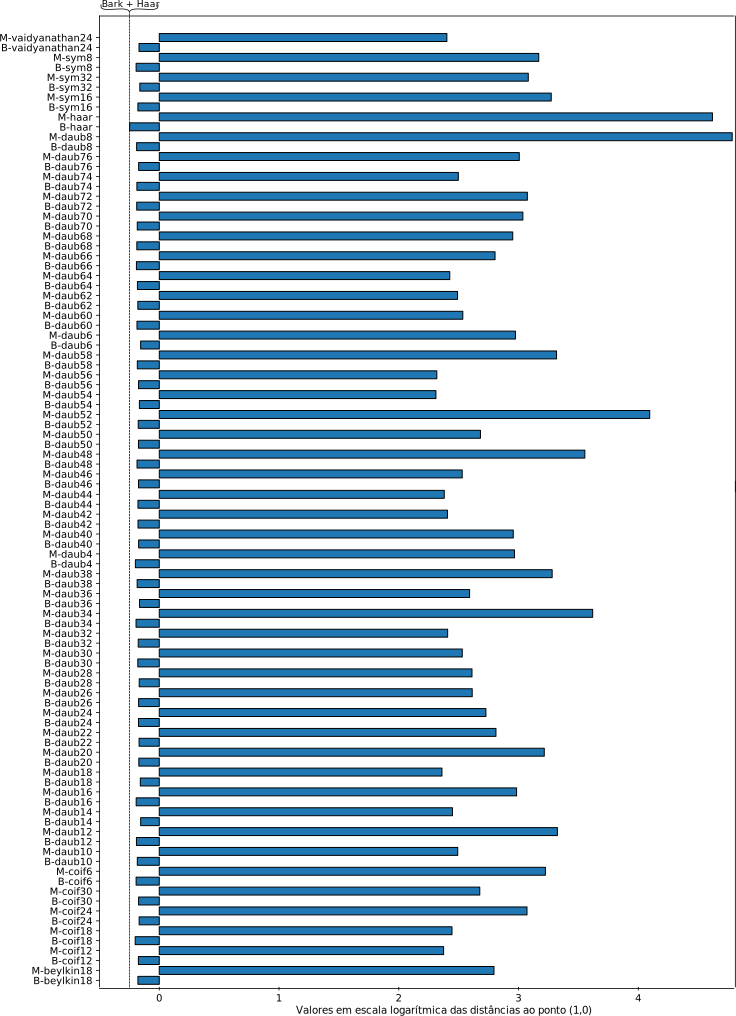
\includegraphics[width=0.99\linewidth]{images/results/paraconsistentPlane/ParaconsistentFull}
				\caption{Gráfico completo da distância ao ponto (1,0) no plano paraconsistente.}
				\label{fig:paraconsistentfull}
			\end{figure}
	\chapter{Recursos na web}
		\par Para realização deste trabalho foram produzidos variados textos (este incluso) e códigos. 
		\par Todos os materiais estão disponíveis em:  \href{https://github.com/ensismoebius/mestrado}{https://github.com/ensismoebius/mestrado}.
\end{apendicesenv}